\documentclass[tikz,border=6pt]{standalone}
\usetikzlibrary{arrows.meta}

\begin{document}
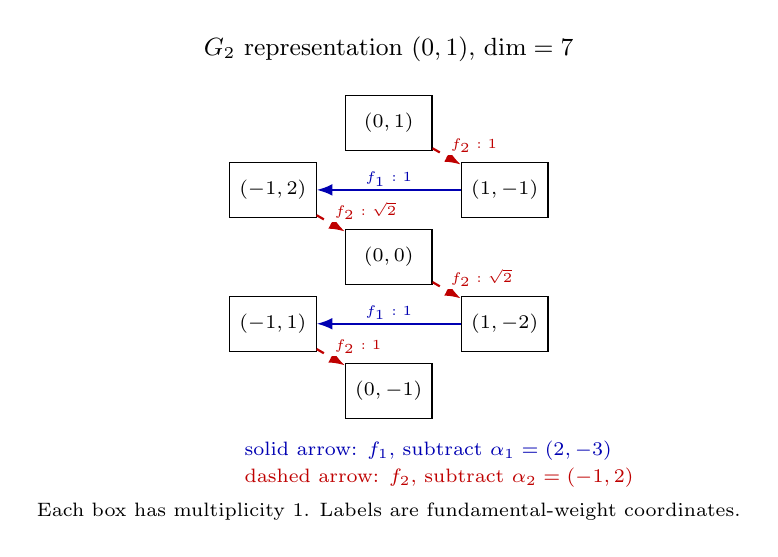
\begin{tikzpicture}[
  x=1.7cm,
  y=1.7cm,
  weight/.style={draw=black, fill=white, minimum width=11mm, minimum height=7mm, inner sep=1pt, font=\scriptsize},
  coef/.style={fill=white, inner sep=1pt, font=\tiny},
  edgeone/.style={blue!70!black, line width=0.8pt, -{Latex[length=2mm]}},
  edgetwo/.style={red!75!black, dashed, line width=0.8pt, -{Latex[length=2mm]}}
]
\node[font=\small] at (0,1.55) {$G_2$ representation $(0,1)$, $\dim=7$};

\node[weight] (p01) at (0,1) {$(0,1)$};
\node[weight] (p1m1) at (0.866,0.5) {$(1,-1)$};
\node[weight] (p1m2) at (0.866,-0.5) {$(1,-2)$};
\node[weight] (p0m1) at (0,-1) {$(0,-1)$};
\node[weight] (m1p1) at (-0.866,-0.5) {$(-1,1)$};
\node[weight] (m1p2) at (-0.866,0.5) {$(-1,2)$};
\node[weight] (zero) at (0,0) {$(0,0)$};

\draw[edgetwo] (p01) -- node[coef, above right] {$f_2:1$} (p1m1);
\draw[edgetwo] (m1p2) -- node[coef, above right] {$f_2:\sqrt{2}$} (zero);
\draw[edgetwo] (zero) -- node[coef, above right] {$f_2:\sqrt{2}$} (p1m2);
\draw[edgetwo] (m1p1) -- node[coef, above right] {$f_2:1$} (p0m1);

\draw[edgeone] (p1m1) -- node[coef, above] {$f_1:1$} (m1p2);
\draw[edgeone] (p1m2) -- node[coef, above] {$f_1:1$} (m1p1);

\node[font=\scriptsize, blue!70!black, anchor=west] at (-1.15,-1.45) {solid arrow: $f_1$, subtract $\alpha_1=(2,-3)$};
\node[font=\scriptsize, red!75!black, anchor=west] at (-1.15,-1.65) {dashed arrow: $f_2$, subtract $\alpha_2=(-1,2)$};
\node[font=\scriptsize] at (0,-1.9) {Each box has multiplicity $1$. Labels are fundamental-weight coordinates.};
\end{tikzpicture}
\end{document}
